\documentclass[xcolor={dvipsnames}]{beamer}

%\usetheme{default}
\usetheme{Boadilla}
%\usetheme{Pittsburgh}

\usecolortheme{beaver}

\setbeamercovered{transparent}
\setbeamertemplate{navigation symbols}{} %remove navigation symbols

\usepackage[english]{babel}
\usepackage[latin1]{inputenc}
\usepackage{times}
\usepackage[T1]{fontenc}

\usepackage{tikz,amsmath,verbatim,wasysym}

% math macros
\newcommand\bb{\mathbf{b}}
\newcommand\bbf{\mathbf{f}}
\newcommand\bn{\mathbf{n}}
\newcommand\bq{\mathbf{q}}
\newcommand\bs{\mathbf{s}}
\newcommand\bu{\mathbf{u}}
\newcommand\bv{\mathbf{v}}
\newcommand\bx{\mathbf{x}}
\newcommand\by{\mathbf{y}}
\newcommand\bz{\mathbf{z}}

\newcommand\bF{\mathbf{F}}
\newcommand\bQ{\mathbf{Q}}
\newcommand\bU{\mathbf{U}}
\newcommand\bV{\mathbf{V}}
\newcommand\bX{\mathbf{X}}

\newcommand\RR{\mathbb{R}}

\newcommand{\DDt}[1]{\ensuremath{\frac{d #1}{d t}}}
\newcommand{\ddt}[1]{\ensuremath{\frac{\partial #1}{\partial t}}}

\newcommand\Div{\nabla\cdot}
\newcommand\eps{\epsilon}
\newcommand\grad{\nabla}
\newcommand{\ip}[2]{\ensuremath{\left<#1,#2\right>}}


\title[Computing glacier geometry]{Computing glacier geometry \\ in nonlinear complementarity problem form}

\author{Ed Bueler}

\institute[UAF] % (optional, but mostly needed)
{
  Dept of Mathematics and Statistics, and Geophysical Institute\\
  University of Alaska Fairbanks \\
  \tiny (\emph{funded by NASA Modeling, Analysis, and Prediction program})%
}

\date[Copper Mtn 2016]{Copper Mountain Iterative March 2016}


\begin{document}
\graphicspath{{../../talks-public/commonfigs/}}

\begin{frame}
  \titlepage
\end{frame}


\begin{frame}{outline}
  \tableofcontents
\end{frame}


\section{NCPs and VIs, a superficial intro}

\begin{frame}{nonlinear complementarity problems (NCP)}

\begin{itemize}
\item in finite dimensions, an NCP is to find $\bz\in\RR^n$ for which
\begin{equation}
\bz \ge 0, \quad \bF(\bz) \ge 0, \quad \bz^\top \bF(\bz) = 0, \label{ncp}
\end{equation}
given a differentiable map $\bF:\RR^n \to \RR^n$
\end{itemize}

\begin{columns}
\begin{column}{0.45\textwidth}
\begin{itemize}
\footnotesize
\item example: given $\psi(x)$, the 1d \alert{obstacle problem} is to find $u(x)$ so that $u(x) \ge \psi(x)$ and $-u''(x) = 0$ where $u>\psi$
\item \dots think about the gap \dots
\item discretized and in form \eqref{ncp}:
\begin{align*}
{\color{red} z_j} &= u_j - \psi(x_j) \\
{\color{ForestGreen} F_j}(\bz) &= - \frac{z_{j+1} - 2 z_j + z_{j-1}}{\Delta x^2} - \psi_j''
\end{align*}
\end{itemize}
\end{column}
\begin{column}{0.55\textwidth}
\includegraphics[width=\textwidth,keepaspectratio=true]{obstacle1d}

\medskip
\includegraphics[width=\textwidth,keepaspectratio=true]{ncp1d}
\end{column}
\end{columns}
\end{frame}


\begin{frame}{variational inequalities (VI)}

\begin{itemize}
\item in finite dimensions, a VI is to find $\bu\in\mathcal{K}$, where $\mathcal{K}\subseteq \RR^n$ is convex and closed, for which
\begin{equation}
     \ip{\bF(\bu)}{\bv-\bu} \ge 0 \quad \forall \bv \in \mathcal{K},
\end{equation}
given a differentiable map $\bF:\RR^n \to \RR^n$
\end{itemize}

\begin{columns}
\begin{column}{0.4\textwidth}
\small
\begin{itemize}
\item obstacle problem:

$\mathcal{K} = \{{\color{red} u_j} \ge {\color{blue} \psi(x_j)}\}$ and
  $$F_j(\bu) = - \frac{u_{j+1} - 2 u_j + u_{j-1}}{\Delta x^2}$$
\end{itemize}
\end{column}
\begin{column}{0.6\textwidth}
\includegraphics[width=\textwidth,keepaspectratio=true]{vi1d}
\end{column}
\end{columns}\end{frame}


\begin{frame}{NCP/VI generalities}

\begin{itemize}
\item in finite dimensions when $\mathcal{K}$ is a cone (as in this talk):
\begin{center}
\alert{NCP $\iff$ VI}
\end{center}
\item both 
  \begin{itemize}
  \item[$\circ$]  generalize nonlinear eqns ``$\bF(\bz)=0$'' to allow constraints on $\bz$
  \item[$\circ$]  are nonlinear, even if $\bF$ is linear or affine
  \item[$\circ$]  in practice: need iterative approach to solve
  \end{itemize}
\item constrained optimization $\implies$ VI $\iff$ NCP
  \begin{itemize}
  \item[$\circ$]  i.e.~find minimum of $\Phi[\bz]$ from $\mathcal{K}$
  \item[$\circ$]  symmetric Jacobian/Hessian in optimizations ($J = \bF' = \Phi''$)
  \end{itemize}
\item \emph{but}: NCP and VI arising in glacier problems are \alert{not} optimizations
\end{itemize}
\end{frame}


\begin{frame}{numerical support}

libraries with scalable support for NCP and/or VI:
\begin{itemize}
\item  PETSc SNES
  \begin{itemize}
  \item[$\circ$]  does not assume optimization
  \item[$\circ$]  used this in all results later in talk
  \end{itemize}
\item  TAO
  \begin{itemize}
  \item[$\circ$]  in PETSc release
  \item[$\circ$]  separate code from SNES
  \end{itemize}
\item  DUNE
  \begin{itemize}
  \item[$\circ$]  used in 2011 \dots still maintained?
  \end{itemize}
\end{itemize}
\end{frame}


\begin{frame}{algorithms}

two Newton line search NCP methods in PETSc SNES:\footnote{Benson \& Munson (2006), and Barry Smith}
\begin{itemize}
\item  ``reduced-space'' = \alert{RS}
    \begin{itemize}
    \item[$\circ$] active set $\mathcal{A} = \{i \,:\, z_i = 0 \text{ and } F_i(\bz) > 0\}$
    \item[$\circ$] inactive set $\mathcal{I} = \{i \,:\, z_i > 0 \text{ or } F_i(\bz) \le 0\}$
    \item[$\circ$] \emph{algorithm}: compute Newton step $\bs^k$ by
     $$\big[J(\bz^k)\big]_{\mathcal{I}^k,\mathcal{I}^k} \bs_{\mathcal{I}^k} = - \bF_{\mathcal{I}^k}(\bz^k)$$
     then do projected line search onto $\{\bz\ge 0\}$
    \end{itemize}
\item  ``semi-smooth'' = \alert{SS}
    \begin{itemize}
    \item[$\circ$] ``NCP function'':
\vspace{-2mm}
    $$\phi(a,b)=0 \quad \iff \quad a\ge 0, b\ge 0, ab=0$$
    \item[$\circ$] \emph{algorithm}: compute Newton step $\bs^k$ by
    $$L^k \bs^k = - \phi(\bz^k,\bF^k(\bz^k))$$
    where $L^k$ is element of $\partial_B \phi(\bz^k,\bF^k(\bz^k))$; then do line search
    \end{itemize}
\end{itemize}
\end{frame}


\AtBeginSection[] % Do nothing for \section*
{
\begin{frame}<beamer>
\frametitle{outline}
\tableofcontents[currentsection]
\end{frame}
}

\section{glacier geometry-evolution models}

\begin{frame}{glacier (and ice sheet) notation}

\begin{center}
\includegraphics[width=0.5\textwidth,keepaspectratio=true]{groundedscheme}
\end{center}

\begin{itemize}
\item unknowns:
  \begin{itemize}
  \item[$\circ$]  $h(t,x,y)$ ice thickness \hfill \dots also $s=h+b$ surface elevation
  \item[$\circ$]  $\bU(t,x,y,z) = \left<u,v,w\right>$ ice velocity
  \end{itemize}
\item \only<1>{data}\only<2>{\alert{uncertain ``data'' from other models}}:
  \begin{itemize}
  \item[$\circ$]  $b(x,y)$ bed elevation \only<2>{\quad \alert{? \quad \dots improving for ice sheets}}
  \item[$\circ$]  $a(t,x,y)$ surface mass balance  \only<2>{\quad \alert{???}}
    \begin{itemize}
    \item accumulation/ablation function; $=$ precipitation $-$ melt
    \end{itemize}
  \end{itemize}
\item ignored in this talk:
  \begin{itemize}
  \item[$\circ$]  conservation of energy (temperature/enthalpy)
  \item[$\circ$]  floating ice
  \item[$\circ$]  solid-earth deformation
  \end{itemize}
\end{itemize}
\end{frame}


\begin{frame}{solve coupled mass and momentum equations}

\begin{itemize}
\item my goal: better ice sheet models \only<2>{\hfill\alert{\dots than PISM}}
  \begin{itemize}
  \item[$\circ$] suitable for long/paleo ($\sim 100$ka) and high res ($\sim 1$ km) \only<2>{\hfill\alert{$\sim\checkmark$}}
  \item[$\circ$] without time-splitting \only<2>{\hfill\alert{\large\frownie{}}}
  \item[$\circ$] with explicit time-step restrictions \only<2>{\hfill\alert{\large\frownie{}}}
  \end{itemize}
\item here just two coupled conservations:
  \begin{itemize}
  \item[$\circ$]  \alert{mass conservation}
\begin{equation*}
h_t + \Div\bq = a
\end{equation*}
    \begin{itemize}
    \vspace{-5mm}
    \item $\bq = h\, \ip{\bar u}{\bar v}$ is vertically-integrated ice flux
    \item equivalent to ``surface kinematical equation'' (ice incompressible)
    \end{itemize}
  \item[$\circ$]  \alert{momentum conservation}
\begin{equation*}
  \nabla \cdot \bU = 0 \qquad \text{and} \qquad - \nabla \cdot \tau_{ij} + \nabla p - \rho\, \mathbf{g} = 0
\end{equation*}
    \begin{itemize}
    \vspace{-5mm}
    \item incompressible power-law Stokes ($D_{ij} = A \tau^{\nu-1} \tau_{ij}$ for $\nu=3$)
    \item geometry ($h$ \& $b$) enters into boundary conditions
    \end{itemize}
  \end{itemize}
\end{itemize}
\end{frame}


\begin{frame}{many possible momentum equations}

  \begin{itemize}
  \scriptsize
  \item[$\circ$] incompressible power-law Stokes
\begin{equation*}
  \nabla \cdot \bU = 0 \qquad \text{and} \qquad - \nabla \cdot \tau_{ij} + \nabla p - \rho\, \mathbf{g} = 0
\end{equation*}
  \item[$\circ$] Blatter-Pattyn equations [$\eta$ is effective viscosity]
$$-\Div \left[\eta \begin{pmatrix}
4 u_x+2v_y & u_y+v_x   & u_z \\
u_y+v_x    & 2u_x+4v_y & v_z
\end{pmatrix} \right] + \rho g \grad s = 0$$
  \item[$\circ$] shallow shelf approximation (SSA)
$$-\Div \left[\bar \eta h \begin{pmatrix}
4 \bar u_x+2\bar v_y & \bar u_y+\bar v_x   \\
\bar u_y+\bar v_x    & 2\bar u_x+4\bar v_y
\end{pmatrix} \right] - \tau_b + \rho g h \grad s = 0$$
  \item[$\circ$] non-sliding shallow ice approximation (SIA)
$$-\frac{\partial}{\partial z} \left[\eta \begin{pmatrix}
u_z \\
v_z
\end{pmatrix} \right] + \rho g \grad s = 0
\qquad \to \qquad
\ip{\bar u}{\bar v} = -\Gamma h^{\nu+2} |\grad s|^{\nu-1} \grad s$$
  \end{itemize}

\begin{itemize}
\item slow fluid momentum-conservation models all
\begin{center}
\alert{generate velocity $\bU=\left<u,v,w\right>$ from geometry $h$ \& $b$}
\end{center}
\item momentum equations are $\mathcal{M}(\bU,h,b)=0$
\end{itemize}
\end{frame}


\begin{frame}{a fluid layer in a climate}

\begin{center}
\includegraphics[width=0.7\textwidth,keepaspectratio=true]{cartoon-wclimate}
\end{center}

\vspace{-7mm}
\begin{itemize}
\item mass conservation equation on last slide applies to broader class:
  \begin{center}
  \alert{a fluid layer on a substrate, evolving in a climate}
  \end{center}
\item mass conservation PDE:
\begin{equation}
h_t + \Div\bq = {\color{blue} a}  \tag{$\ast$} \label{mc}
\end{equation}
    \begin{itemize}
    \vspace{-4mm}
    \item[$\circ$] $h$ is a thickness so $h\ge 0$
    \item[$\circ$] \eqref{mc} applies only where $h>0$
    \item[$\circ$] signed source ${\color{blue} a}$ is the ``climate''
    \end{itemize}
\end{itemize}
\end{frame}


\begin{frame}{fluid layers in climates}

\includegraphics[width=0.4\textwidth,keepaspectratio=true]{polaris}
\hfill
\includegraphics[width=0.45\textwidth,keepaspectratio=true]{supp4rignot-small}

\small glaciers \hfill sea ice (\& ice shelves)

\medskip
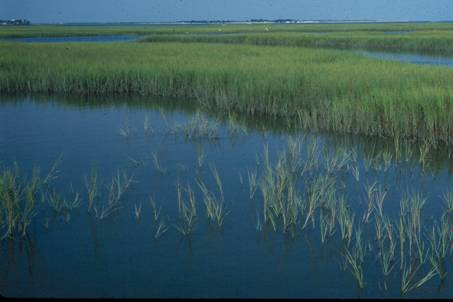
\includegraphics[width=0.41\textwidth,keepaspectratio=true]{marsh-water}
\hfill
\includegraphics<1>[width=0.42\textwidth,keepaspectratio=true]{tsunami-sendai}
\only<2>{\small \vspace{-3.7mm}\begin{minipage}[t]{0.4\textwidth} surface hydrology, subglacial hydrology, \dots \end{minipage} }

\small tidewater marsh \hfill \only<1>{tsunami inundation}
\end{frame}


\section{every time-step is free-boundary problem}

\newcommand{\singletsmc}{\frac{h^\ell - h^{\ell-1}}{\Delta t} + \Div \bq^\ell = a^\ell}
\begin{frame}{semi-discretize in time}

\begin{itemize}
\item semi-discretize coupled model (e.g.~$h^\ell(x,y) \approx h(t^\ell,x,y)$)
$$\begin{matrix}
 h_t + \Div\bq = a \\
 \phantom{foo} \\
 \mathcal{M}(\bU,h,b) = 0
\end{matrix} \qquad \to \qquad \begin{matrix}
 \only<1>{\singletsmc} \only<2>{\alert{\singletsmc}} \\
 \phantom{foo} \\
 \mathcal{M}(\bU^\ell,h^\ell,b) = 0
\end{matrix}$$
\item coupling also through $\bq=\bq(\bU,h,\grad h)$
\item details of flux $\bq^\ell$ and source $a^\ell$ come from time-stepping scheme
        \begin{itemize}
        \item[$\circ$] backward-Euler shown
        \item[$\circ$] could use other $\theta$-methods or BDFs
        \end{itemize}
\item<2> \alert{need to weakly-pose single time-step mass conservation equation incorporating $h^\ell\ge 0$ constraint \dots it generates the free boundary}
\end{itemize}
\end{frame}


\begin{frame}{mass conservation: VI form}

\begin{itemize}
\item single time-step mass conservation equation
\begin{equation}
\frac{h^\ell - h^{\ell-1}}{\Delta t} + \Div \bq^\ell = a^\ell \tag{MC} \label{mcstrong}
\end{equation}
\item from now on: assume $\bq=0$ on any open set where $h=0$
    \begin{itemize}
    \item[$\circ$] because it is a flowing \emph{layer}
    \end{itemize}
\item first weak formulations of \ref{mcstrong} for glaciers were VIs
    \begin{itemize}
    \item[$\circ$] Calvo et al (2002): SIA 1d flat bed
    \item[$\circ$] Jouvet \& Bueler (2012): SIA 2d general bed steady
    \end{itemize}
\item define $\mathcal{K} = \left\{v \in W^{1,p}(\Omega) \,\Big|\, v\ge 0\right\}$
\item VI form of MC: find $h^\ell\in\mathcal{K}$
    $$\int_\Omega h^\ell (v - h^\ell) - \Delta t\, \bq^\ell \cdot \grad(v - h^\ell) \ge \int_\Omega \left(h^{\ell-1} + \Delta t\, a^\ell\right) (v - h^\ell)$$
for all $v \in \mathcal{K}$
\end{itemize}
\end{frame}


\begin{frame}{mass conservation: NCP form}

\begin{itemize}
\item recall general NCP is
  $$\bz \ge 0, \quad \bF(\bz) \ge 0, \quad \bz^\top \bF(\bz) = 0$$
\item define
    $$F(h) = h^\ell - h^{\ell-1} + \Delta t\, \Div \bq^\ell - \Delta t\, a^\ell$$
\item NCP form of MC:
   $$h^\ell \ge 0, \quad F(h^\ell) \ge 0, \quad h^\ell F(h^\ell) = 0$$
\item setwise statements from the NCP:
    \begin{itemize}
    \item[$\circ$] where $h^\ell > 0$,
        $$F(h^\ell) = 0 \qquad \iff \qquad \text{strong form MC}$$
        \vspace{-4mm}
        \begin{itemize}
        \item interior condition
        \end{itemize}
    \item[$\circ$] where $h^\ell = 0$,
        $$h^{\ell-1} + \Delta t\, a^\ell \le 0$$
        \vspace{-4mm}
        \begin{itemize}
        \item says ``surface mass balance is negative enough during time step to remove old thickness''
        \end{itemize}
    \end{itemize}
\end{itemize}
\end{frame}


\section{proposed approach: FVE discretization + Newton + continuation}

\begin{frame}{finite volume element (FVE) discretization}

\begin{itemize}
\item from now on in this talk: steady case ($\Delta t = \infty$)
\item for FVE, see Cai (1990) and Ewing, Lin, \& Lin (2002)
\item thickness $h(x,y)$ lives in $Q^1$ FEM space $\subset W^{1,\nu+1}(\Omega)$
    \begin{itemize}
    \item[$\circ$] structured grid for now; $h$ bilinear on elements $\square_{j,k}$
    \end{itemize}
\item mass conservation $\iff$ control-volume integral on $V=V_{j,k}$:
    $$\Div \bq = a \qquad \iff \qquad \int_{\partial V} \bq \cdot \bn \,ds \stackrel{\ast}{=} \int_V a \,dx\,dy$$ 
\item \emph{thus}: a finite element method where $\ast$ is the weak form
    \begin{itemize}
    \item[$\circ$] \emph{or}: Petrov-Galerkin FEM with $\chi_V$ as test function
    \item[$\circ$] no symmetry in weak form \dots no loss
    \end{itemize}
\end{itemize}

\begin{center}
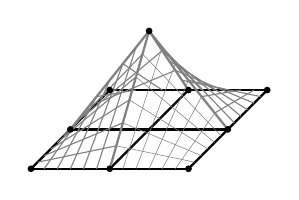
\begin{tikzpicture}[scale=0.25]
  % strong grid around elements
  \draw[thick] (0,0) -- (8,0);
  \draw[thick] (2,2) -- (10,2);
  \draw[thick] (4,4) -- (12,4);
  \draw[thick] (0,0) -- (4,4);
  \draw[thick] (4,0) -- (8,4);
  \draw[thick] (8,0) -- (12,4);

  \def\ytop{7};

  % tent lines
  \draw[gray,thick] (6,\ytop) -- (4,0);
  \draw[gray,thick] (6,\ytop) -- (2,2);
  \draw[gray,thick] (6,\ytop) -- (10,2);
  \draw[gray,thick] (6,\ytop) -- (8,4);

  \def\dx{(10.0-6.0)/6};
  \def\dy{(2.0-\ytop)/6};
  \foreach \jj in {1,...,5}
  {
       \draw[gray,very thin] ({6+\jj*\dx},{\ytop+\jj*\dy}) -- ({4+(4/6)*\jj},0.0);
  }

  \def\dx{(4.0-6.0)/6};
  \def\dy{(0.0-\ytop)/6};
  \foreach \jj in {1,...,5}
  {
       \draw[gray,very thin] ({6+\jj*\dx},{\ytop+\jj*\dy}) -- ({10-(2/6)*\jj},{2-(2/6)*\jj});
  }

  \def\dx{(2.0-6.0)/6};
  \def\dy{(2.0-\ytop)/6};
  \foreach \jj in {1,...,5}
  {
       \draw[gray,thin] ({6+\jj*\dx},{\ytop+\jj*\dy}) -- ({4-(4/6)*\jj},0.0);
  }

  \def\dx{(4.0-6.0)/6};
  \def\dy{(0.0-\ytop)/6};
  \foreach \jj in {1,...,5}
  {
       \draw[gray,thin] ({6+\jj*\dx},{\ytop+\jj*\dy}) -- ({2-(2/6)*\jj},{2-(2/6)*\jj});
  }

  \def\dx{(10.0-6.0)/6};
  \def\dy{(2.0-\ytop)/6};
  \foreach \jj in {1,...,5}
  {
       \draw[gray,thin] ({6+\jj*\dx},{\ytop+\jj*\dy}) -- ({8+(4/6)*\jj},4.0);
  }

  \def\dx{(8.0-6.0)/6};
  \def\dy{(4.0-\ytop)/6};
  \foreach \jj in {1,...,5}
  {
       \draw[gray,thin] ({6+\jj*\dx},{\ytop+\jj*\dy}) -- ({10+(2/6)*\jj},{2+(2/6)*\jj});
  }

  \def\dx{(2.0-6.0)/3};
  \def\dy{(2.0-\ytop)/3};
  \foreach \jj in {1,...,2}  % reduce clutter
  {
       \draw[gray,thin] ({6+\jj*\dx},{\ytop+\jj*\dy}) -- ({8-(4/3)*\jj},4.0);
  }

  \def\dx{(8.0-6.0)/3};
  \def\dy{(4.0-\ytop)/3};
  \foreach \jj in {1,...,2}
  {
       \draw[gray,thin] ({6+\jj*\dx},{\ytop+\jj*\dy}) -- ({2+(2/3)*\jj},{2+(2/3)*\jj});
  }

  % nodes in base plane
  \filldraw (0,0) circle (4pt);
  \filldraw (4,0) circle (4pt);
  \filldraw (8,0) circle (4pt);
  \filldraw (2,2) circle (4pt);
  %\filldraw (6,2) circle (4pt);   % (x_j,y_k) is at (6,2)
  \filldraw (10,2) circle (4pt);
  \filldraw (4,4) circle (4pt);
  \filldraw (8,4) circle (4pt);
  \filldraw (12,4) circle (4pt);

  % node at tent top
  \filldraw (6,\ytop) circle (4pt);
\end{tikzpicture}
\qquad \qquad
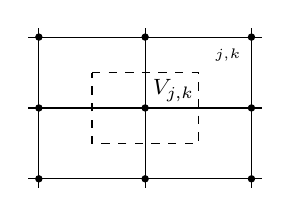
\begin{tikzpicture}[scale=0.45]
  % strong grid around elements
  \draw (-0.3,0) -- (6.3,0);
  \draw (-0.3,2) -- (6.3,2);
  \draw (-0.3,4) -- (6.3,4);
  \draw (0,-0.25) -- (0,4.25);
  \draw (3,-0.25) -- (3,4.25);
  \draw (6,-0.25) -- (6,4.25);
  % nodes
  \filldraw (0,0) circle (2.5pt);
  \filldraw (3,0) circle (2.5pt);
  \filldraw (6,0) circle (2.5pt);
  \filldraw (0,2) circle (2.5pt);
  \filldraw (3,2) circle (2.5pt);
  \filldraw (6,2) circle (2.5pt);
  \filldraw (0,4) circle (2.5pt);
  \filldraw (3,4) circle (2.5pt);
  \filldraw (6,4) circle (2.5pt);
  % outline control volume
  \draw[dashed] (1.5,3) -- (4.5,3) -- (4.5,1) -- (1.5,1) -- cycle;
  % label elements and control volume
  \draw (3.8,2.5) node {\footnotesize $V_{j,k}$};
  \draw (5.35,3.5) node {\scriptsize $\square_{j,k}$};
\end{tikzpicture}
\end{center}

\end{frame}


\begin{frame}{quadrature and upwinding}

\begin{itemize}
\item FD schemes fit into above FVE framework
  \begin{itemize}
  \item[$\circ$] old FD scheme by Mahaffy (1976) fits \dots has weird quadrature
  \item[$\circ$] improved convergence comes from using quadrature points below:
  \end{itemize}
\begin{center}
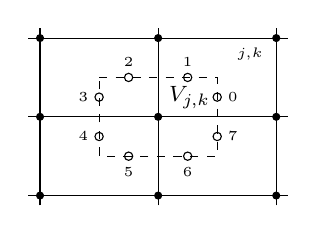
\begin{tikzpicture}[scale=0.5]
  % strong grid around elements
  \draw (-0.3,0) -- (6.3,0);
  \draw (-0.3,2) -- (6.3,2);
  \draw (-0.3,4) -- (6.3,4);
  \draw (0,-0.25) -- (0,4.25);
  \draw (3,-0.25) -- (3,4.25);
  \draw (6,-0.25) -- (6,4.25);
  % nodes
  \filldraw (0,0) circle (2.5pt);
  \filldraw (3,0) circle (2.5pt);
  \filldraw (6,0) circle (2.5pt);
  \filldraw (0,2) circle (2.5pt);
  \filldraw (3,2) circle (2.5pt);
  \filldraw (6,2) circle (2.5pt);
  \filldraw (0,4) circle (2.5pt);
  \filldraw (3,4) circle (2.5pt);
  \filldraw (6,4) circle (2.5pt);
  % outline control volume
  \draw[dashed] (1.5,3) -- (4.5,3) -- (4.5,1) -- (1.5,1) -- cycle;
  % mark quadrature points
  \draw (4.5,2.5) circle (3.0pt) node[shift={(0.2,0.0)}] {\tiny 0};
  \draw (3.75,3)  circle (3.0pt) node[shift={(0.0,0.2)}] {\tiny 1};
  \draw (2.25,3)  circle (3.0pt) node[shift={(0.0,0.2)}] {\tiny 2};
  \draw (1.5,2.5) circle (3.0pt) node[shift={(-0.2,0.0)}] {\tiny 3};
  \draw (1.5,1.5) circle (3.0pt) node[shift={(-0.2,0.0)}] {\tiny 4};
  \draw (2.25,1)  circle (3.0pt) node[shift={(0.0,-0.2)}] {\tiny 5};
  \draw (3.75,1)  circle (3.0pt) node[shift={(0.0,-0.2)}] {\tiny 6};
  \draw (4.5,1.5) circle (3.0pt) node[shift={(0.2,0.0)}] {\tiny 7};
  % label elements and control volume
  \draw (3.8,2.5) node {\footnotesize $V_{j,k}$};
  \draw (5.35,3.6) node {\scriptsize $\square_{j,k}$};
\end{tikzpicture}
\end{center}
\item a bit of upwinding improves convergence on non-flat beds
  \begin{itemize}
  \item[$\circ$] \dots even though this is a fully-implicit approach
  \item[$\circ$] tested on bedrock-step exact solution (Jarosch et al 2013)
  \item[$\circ$] details out of scope here
  \end{itemize}
\end{itemize}
\end{frame}


\begin{frame}{restrict to SIA}

\begin{itemize}
\item from now on: restrict to nonsliding SIA
\item steady SIA mass conservation equation (SIA MC)
    $$\Div \bq = a, \qquad \bq = - \Gamma h^{\nu+2} |\grad s|^{\nu-1} \grad s$$

\vspace{-2mm}
    \begin{itemize}
    \item[$\circ$] recall $s=h+b$
    \item[$\circ$] main idea: these equations are subject to nontrivial constraint $h\ge 0$, so it is an NCP
    \end{itemize}
\end{itemize}
\end{frame}


\begin{frame}{\emph{ad hoc} continuation scheme}

\begin{itemize}
\item for $0 \le \eps \le 1$, regularize $\bq^{(\eps)}$ so that
  \begin{itemize}
  \item[$\circ$] $\bq^{(\eps_0)}$ with $\eps_0=1$ gives classical obstacle problem
    $$\Div \bq^{(\eps_0)} = a \quad \iff \quad - \Div (D_0 \grad s) = a$$
  \item[$\circ$] $\bq^{(\eps_{12})}$ with $\eps_{12}=0$ gives SIA model
    $$\Div \bq^{(\eps_{12})} = a \quad \iff \quad - \Div (\Gamma h^{\nu+2} |\grad s|^{\nu-1} \grad s) = a$$
  \end{itemize}
\item $\eps_{k-1}$ level generates initial $h$ for $\eps_k$ level
\item at each level, want quadratic convergence from Newton
\end{itemize}

\begin{center}
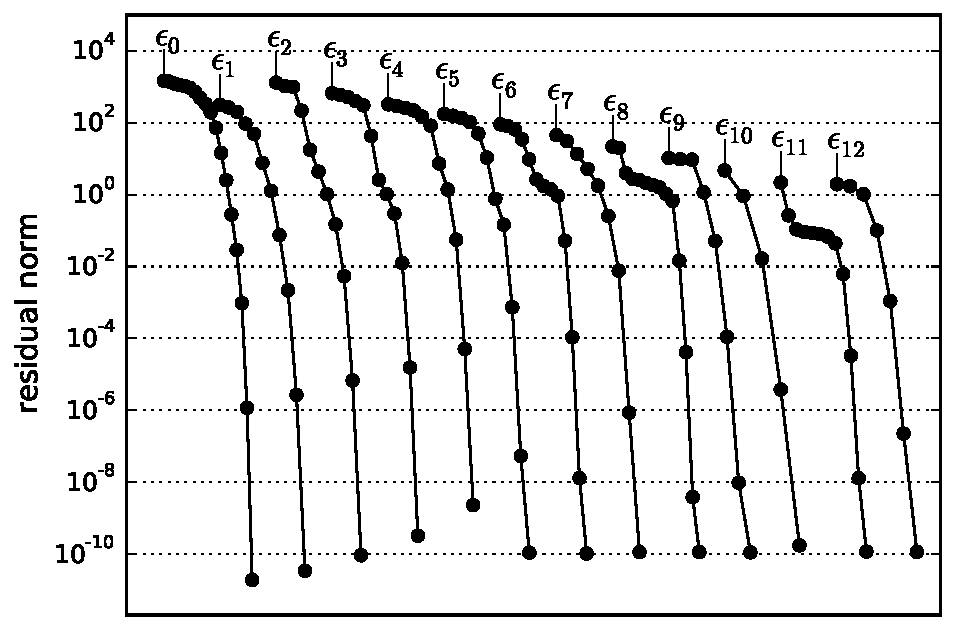
\includegraphics[width=0.4\textwidth,keepaspectratio=true]{newtonconv}
\end{center}
\end{frame}


\section{partial success \dots and the essential difficulty}

\begin{frame}{example: Greenland ice sheet}

\begin{columns}
\begin{column}{0.6\textwidth}
\begin{itemize}
\item \emph{goal}: given steady surface mass balance $a(x,y)$ and bedrock elevation $b(x,y)$, predict the steady geometry $h(x,y)$ of the Greenland ice sheet

\bigskip
\item \emph{method}: solve steady SIA MC NCP
  \begin{itemize}
  \item[$\circ$] reduced-space Newton method
  \item[$\circ$] 900 m structured grid
  \item[$\circ$] $Q^1$ FEs in space
  \item[$\circ$] $N=7\times 10^6$ d.o.f.
  \end{itemize}
\item \emph{result}: at right
  \begin{itemize}
  \item[$\circ$] see Bueler (2016), J.~Glaciol.
  \end{itemize}
\end{itemize}
\end{column}
\begin{column}{0.4\textwidth}
\vspace{-5mm}

\begin{center}
\includegraphics[width=0.95\textwidth,keepaspectratio=true]{grnwinset}
\end{center}
\end{column}
\end{columns}
\end{frame}



\begin{frame}{the essential difficulty: airplanes}

\begin{itemize}
\item actually: \alert{bedrock roughness}
\item improved bed observations $\implies$ worse NCP solver convergence
  \begin{itemize}
  \item[$\circ$] old bed: Bamber (2001)
  \item[$\circ$] new bed: Morlighem (2014)
  \item[$\circ$] results shown for RS; SS is similar
  \end{itemize}
\end{itemize}

\begin{center}
\includegraphics[width=0.6\textwidth,keepaspectratio=true]{rseps}
\end{center}
\end{frame}


\begin{frame}{summary}

  \begin{itemize}
  \item \emph{problem}: fluid layer conservation model \, $h_t + \Div\bq = a$
    \begin{itemize}
    \item[$\circ$]  subject to signed climate $a$
    \item[$\circ$]  thickness $h$ is nonnegative
    \item[$\circ$]  coupled to momentum solver to generate $\bU$ for $\bq$
    \end{itemize}
  \item \emph{goal}:
    \begin{itemize}
    \item[$\circ$]  long time steps wanted
    \end{itemize}
  \item \emph{approach}:
    \begin{itemize}
    \item[$\circ$]  pose single time-step problem weakly as NCP or VI
      \begin{itemize}
      \item  incorporates constraint $h\ge 0$
      \item  approach is very flux-agnostic
      \end{itemize}
    \item[$\circ$]  consider discrete-time, continuous-space problem before coding!
    \item[$\circ$]  solve by scalable constrained-Newton method (PETSc?)
    \end{itemize}
  \item \emph{issues/challenges}:
    \begin{itemize}
    \item[$\circ$]  bed roughness makes convergence hard
    \item[$\circ$]  \alert{every time-step generates near-fractal domain, by free-boundary problem, on which coupled momentum solve must be accurate, especially near the free boundary}
    \end{itemize}
  \end{itemize}

\end{frame}

\end{document}
